\chapter{OBDH}\label{ch:obdh}

The aim of this assignment is to experiment with
a reduced version of an On-Board Data Handling (OBDH) system
implemented on the UPMSat-2 microsatellite.
The OBDH is typically implemented by software,
which is also known as the On-Board Software (OBSW) of the satellite.
In this assignment,
the OBSW reads the MCU temperature using a temperature sensor
that is embedded in the MCU and connected to one of its ADCs.

\section{Software architecture}

The software architecture of the OBSW is depicted in \ref{fig:obdh} The software components are:

\begin{figure}[h]
	\centering{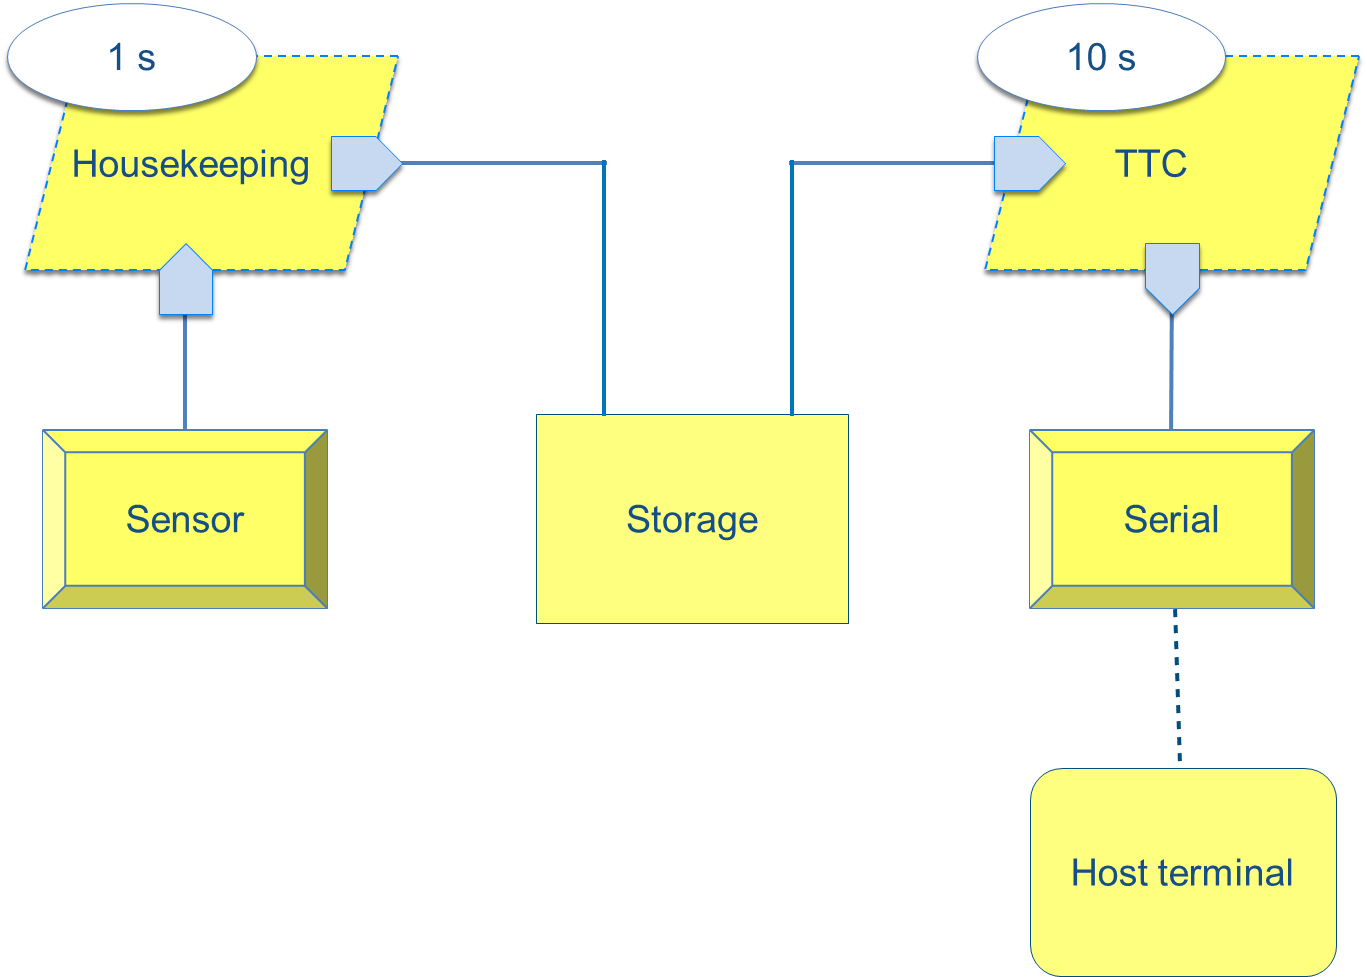
\includegraphics[width=0.8\textwidth,keepaspectratio]{real-time.png}}
	\caption{Software architecture of OBSW.}
	\label{fig:obdh}
\end{figure}

\begin{description}
\item[Telemetry and Telecommand (TTC).] This module is in charge of the communications with the ground station. The ground station is simulated by the Host terminal. It must be activated cyclically with a 10 second period.
\item[Serial.] This module provides a high-level interface to a text console where the measured temperature values can be output.
\item[Housekeeping.] Main component, which performs the basic functionality of the system, i.e. reading a temperature value and storing the value on the Storage component. It must be activated cyclically with a 1 second period.
\item[Sensor.] This module provides a high-level interface to the temperature sensor and deals with all the details of reading the ADC to which the sensor is connected.
\item[Storage.] This component is a data object storing one temperature value, which is written by Housekeeping and read by TTC.
\end{description}

Since the OBC board does not have a text output device, temperature values are sent by a serial line to the ground station. In this way, the radio link between
the satellite and the ground station is simulated.

\section{Serial line connections.}

This scheme makes use of the USB/UART interface cable provided to the students. The USB/ UART cable has a TTL connector that must be connected to the STM32f4 board pins that convey the serial line (UART) signals (figure~\ref{fig:cable}).

\begin{figure}[h]
            \centering{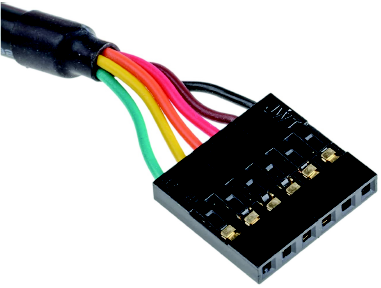
\includegraphics[width=0.3\textwidth,keepaspectratio]{connector.png}}
            \caption{UART cable connector.}
            \label{fig:cable}
\end{figure}

The connections to be made are summarized in the following table (see figure~\ref{fig:board} for the location of the pins on the board):

\begin{table}[htb]
\begin{center}
\begin{tabular}{ll} \hline
Connector pin & Board pin \\ \hline
1 (black) & GND \\
4 (orange) & PB7 \\
5 (yellow) & PB6 \\ \hline
\end{tabular}
\caption{Serial line connections on board.}
\label{tb:connections}
\end{center}
\end{table}

The other end of the interface cable has a USB-A connector that must be plugged to a USB port on the host computer. The values sent to the host computer are displayed using a terminal application that can handle a USB serial port. The host terminal application should be set to taking the USB serial port as input with a transmission rate of 115200 bps and 8N1.

\section{Host terminal application.}\label{sc:term}
\subsection{Windows}

The recommended application to display messages received on the USB serial port is PuTTY. You can download an installation package from \url{https://www.putty.org}.

In order to configure the application, you need first to identify the COM port corresponding to the USB serial line. Open the Device Manager and look at the USB Serial Port entry. The COM port is displayed next to it (e.g. COM 4 in figure~\ref{fig:com}).

\begin{figure}[hbtp!]
            \centering{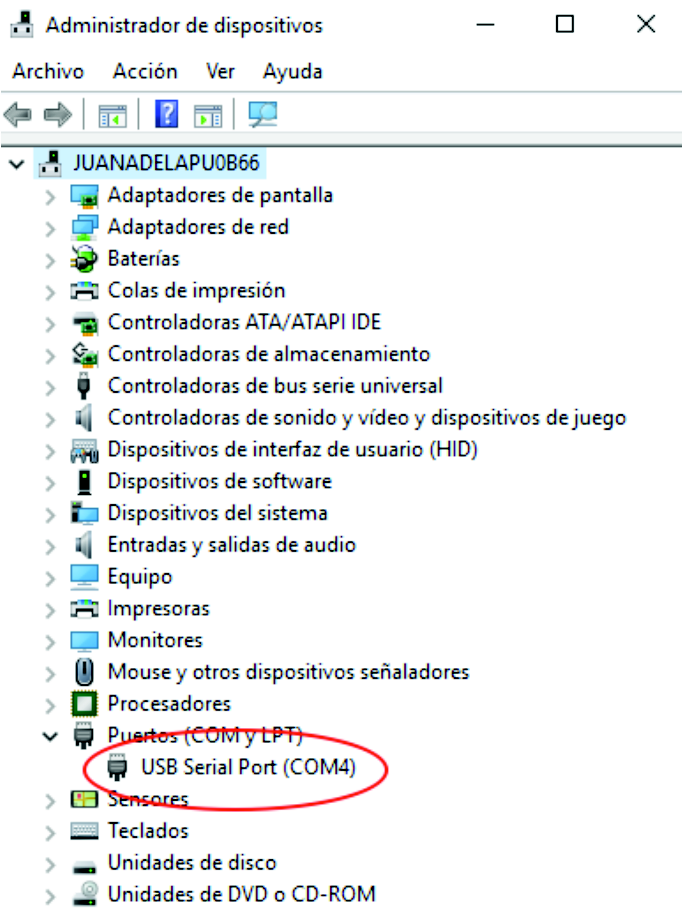
\includegraphics[width=0.6\textwidth,keepaspectratio]{com.png}}
            \caption{Identification of usb serial port.}
            \label{fig:com}
\end{figure}

Now, to set up PuTTY, open the application and set the configuration parameters as shown in figure~\ref{fig:cable}.

\begin{figure}[hbtp!]
            \centering{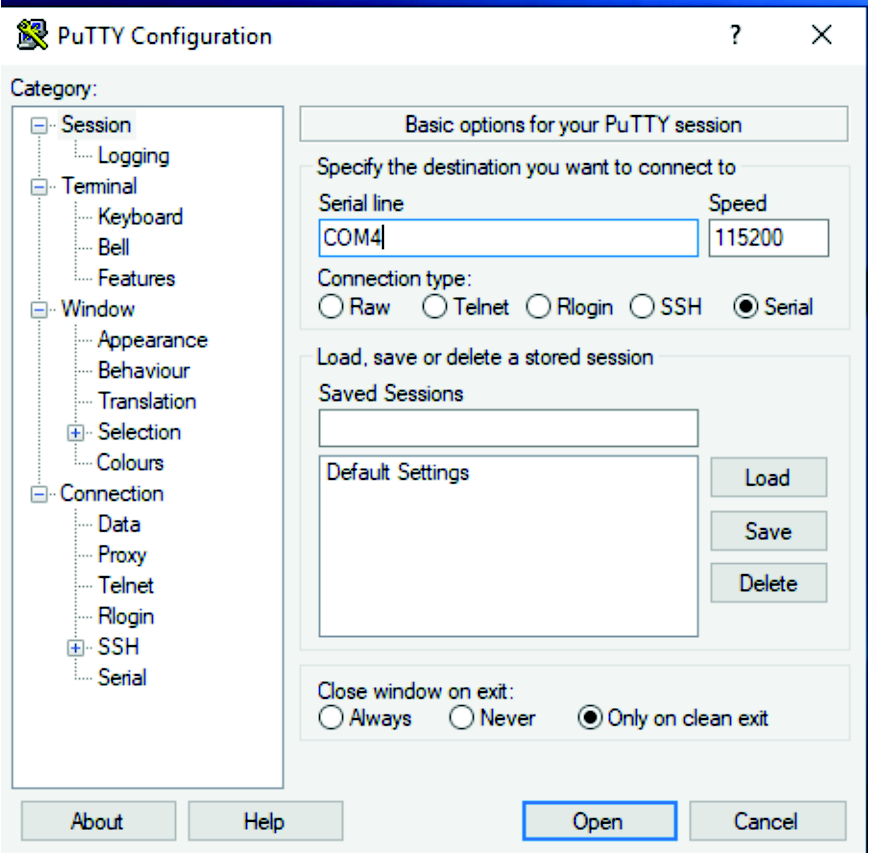
\includegraphics[width=0.6\textwidth,keepaspectratio]{putty.png}}
            \caption{PuTTY configuration.}
            \label{fig:putty}
\end{figure}

\subsection{MacOS}
The recommended application is screen, which is already installed in MacOS.
First you have to identify the USB serial port. Open a terminal window and type

\begin{BVerbatim}
	$ ls /dev | grep -i usb
\end{BVerbatim}

You will get a list of devices like the following:

\begin{BVerbatim}
	cu.usbserial-FTA5I24G
	tty.usbserial-FTA5I24G
\end{BVerbatim}

As you can see, there are two devices for each serial line. You can use any of them, but for reasons not to be discussed here it is better, in general, to use the one starting with cu.

To use the screen application enter the following command:

\begin{BVerbatim}
	$ screen /dev/cu.usbserial-XXXX 115200
\end{BVerbatim}
	
where \texttt{/dev/cu.usbserial-XXXX} is the name of your device.

To exit the application, type CTRL-A and then CTRL-K.

\subsection{GNU Linux}

The recommended application is screen,4 which can be installed in Ubuntu Linux with:

\begin{BVerbatim}
	$ sudo apt install screen
\end{BVerbatim}

In order to identify the USB serial port, type the following command on a terminal:

\begin{BVerbatim}
	$ ls /dev | grep -i usb
\end{BVerbatim}

You will get a result like the following:

\begin{BVerbatim}
	ttyUSB0
\end{BVerbatim}

To use the screen application enter the following command:

\begin{BVerbatim}
	$ screen /dev/ttyUSB0 115200
\end{BVerbatim}

To exit the application, type CTRL-A and then SHIFT-K.

\section{Download the code and study the implementation.}

The implementation code, as initially provided to the students, can be downloaded from \url{https://github.com/STR-UPM/SEU-OBDH-Lab}. Click on Clone or download, download a zip archive, unzip and move to your work directory. The code for this assignment is in the LAB6 folder.

The Housekeeping package is the root element of the housekeeping
subsystem. Its specification consists of one procedure, Initialize, that starts the operation of the component. It has four subpackages:
\begin{description}
\item[Housekeeping] is the root package of the subsystem and contains a concurrent task, Housekeeping\_Task that stores Data in Storage and toggles the blue LED every second.

\item[Housekeeping.Data] contains the definitions of the data types used in the subsystem. The data type Analog\_Data is used to read the ADC, which are integers in the range 0 to 4095 as directly provided by the ADC. The data type State is a record that contains the ADC read and the corresponding timestamp.

These ADC values have to be converted to engineering units. i.e. degrees Celsius, by following the specification of the temperature sensor (se appendix~\ref{ap:sensor}). Raw sensor readings are usually sent to ground station that is in charge of converting them to engineering units.

\item[Housekeeping.Sensor]  contains the details of the temperature sensor. Its specification includes the Initialize and Get procedures. This package uses the Ada Drivers Library to interact with the OBC board hardware.

\item[Housekeeping.Images] includes functions which are used to convert to Strings temperature and timestamp values.
\end{description}

The TTC package is the root of the telecommunications system, which in this version is greatly simplified with respect to a real application. It contains a concurrent task, HK\_Task, which takes measured sensor values from Storage and sends them to the ground station by using Serial every ten seconds. The task also toggles the orange LED.

The Storage package implements the communication between the Housekeeping and TTC subsystems.  Since this object is shared by two concurrent tasks, it is implemented as a protected object, so that its operations are executed in mutual exclusion. There is also conditional synchronization:
the TTC task must wait until there is a fresh value in the store. However, Housekeeping should not wait if the previous value put into Storage has not been consumed, in order not to delay the housekeeping function. In this case, the stored value is overwritten. Notice that this differs from the classical specification of a bounded buffer.

The Serial component is implemented by the Serial.IO package and other packages in the serial\_ports folder. These packages have been adapted from the examples in the Ada Drivers Library. The blocking kind of serial port has been chosen for this project. This means that the task calling the Put operation (TM\_Task) waits on a busy loop until the operation is complete.

The main procedure is OBSW. It calls Housekeeping.Initialize, which initializes the sensor so that Housekeeping\_Task can proceed.
Additionally, the green LEDs is toggled on and off to provide a visual check that the program is running.

Notice that Run, and hence Initialize and OBSW, never return. Therefore the program executes indefinitely, as is common in embedded systems.

\section{Compile and run.}

Open GPS and do the following:
\begin{enumerate}
\item Select Open project on the welcome window. Navigate to the OBSW directory and open the realtime\_housekeeping.gpr project file.
\item Build the executable and load it into the board by clicking on the \hbox{
\includegraphics[width=1.5em]{buildandload.png}} symbol in the tool bar (or select Build $\rightarrow$ Bareboard $\rightarrow$ Flash to board on the top menu).

The program will be compiled, and the executable will be loaded into the board flash memory. After that, the program starts to run on the board (check the blinking LEDs).
\item Connect the serial cable to a USB port on the host computer, if not already done.
\item Identify the serial port name on the host computer and launch the remote terminal application as explained in section~\ref{sc:term}. The sensor measured values together with their respective timestamps will start being displayed on the host application (figure~\ref{fig:output}).
\end{enumerate}

\begin{figure}[h]
            \centering{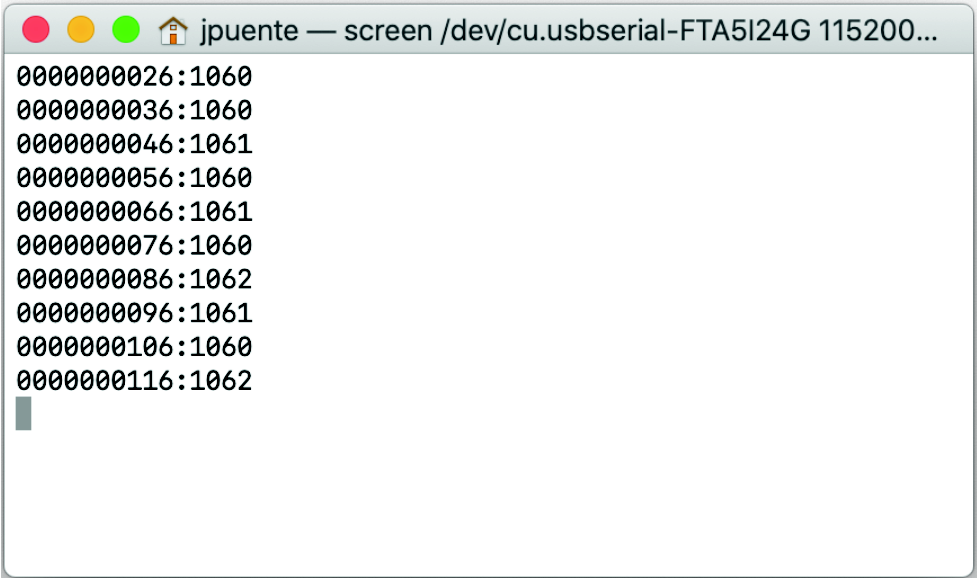
\includegraphics[width=0.6\textwidth,keepaspectratio]{output.png}}
            \caption{Sample output on host terminal.}
            \label{fig:output}
\end{figure}

\section{Make changes to the program.}

You may make change to the provided program in order to make sure
that you understand the logics behind the source code. Proposed change is:

Include the conversion to Celsius in the TTC.Send procedure. Temperature function of HK\_data-converter that can be found in utilities can be used.

\section{Perform a temporal analysis of the system.}\label{sc:ta}

In order to carry out a response-time analysis of the temporal behaviour of the system, you will need to measure the execution time of the task bodies and the protected procedure bodies. A simple loop technique using the standard real-time clock will be enough for this assignment.

An execution time measurement tool is available in the LAB6 directory. In order to use it, perform the following steps:
\begin{enumerate}
\item Open GPS and select Open project on the welcome window. Navigate to the LAB6 directory
and open the wcet\_meter.gpr project file.
\item Build the executable and load into the board in the same way as for the realtime\_housekeeping.
gpr project.
\item Make sure that the serial cable is still connected to the board and the USB port in the host
computer. If the remote terminal application is not open, open it.
\end{enumerate}

A measurement test is executed on the board, and repeated every 60 s. The output of the test is shown on the host terminal application (figure~\ref{fig:wcet}). The output shows the execution times for the bodies of the Housekeeping (HK) and TTC (TC) tasks, as well as the bodies of the protected operations of the Storage object (ST). Notice that a new entry, Get\_Immediate, has been added for the latter in order to avoid the measuring task to get blocked. The new entry is exactly the same as Get but has a True barrier so that it is always open.

\begin{figure}[h]
            \centering{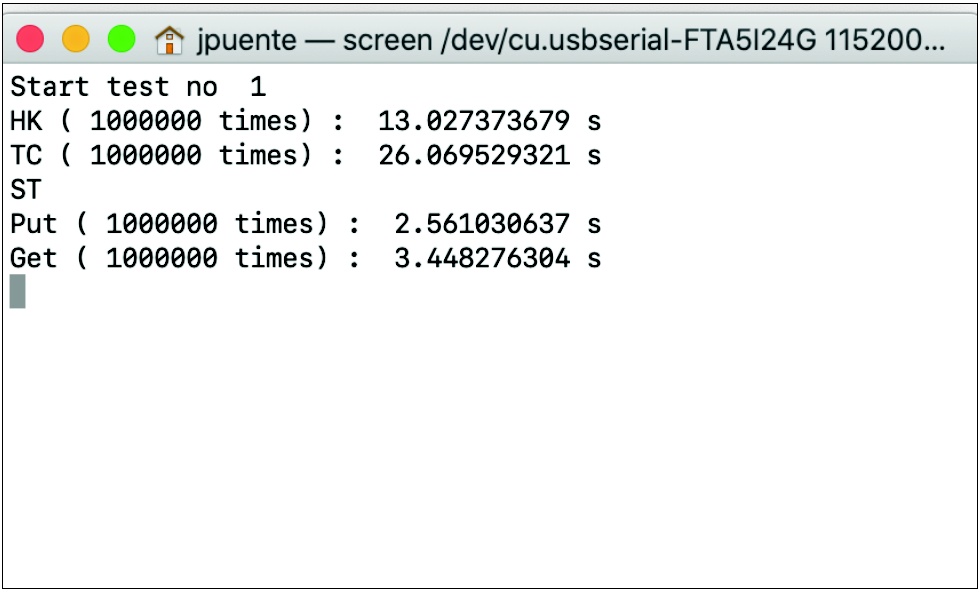
\includegraphics[width=0.6\textwidth,keepaspectratio]{wcet.png}}
            \caption{Output of wcet measurement tool.}
            \label{fig:wcet}
\end{figure}

In the example shown on figure~\ref{fig:wcet}, the HK execution time has been measured $10^{6}$ times, with a total measurement time of 13.02 s. Therefore, the value to be taken for the response time analysis is $13.02\cdot10^{-6}~s = 13.02~\mu${s}, and the same for the other tasks. Take into account that the values measured on your board will probably be slightly different from the above shown.

Once you have an estimate of worst case execution times, apply the RTA equations for computing the worst-case response time and check if all the deadlines are met. The setup for the calculations is shown on table~\ref{tb:wcet}.

\begin{table}[htb]
\begin{center}
\begin{tabular}{|l|r|r|r|r|r|r|r|r|} \hline
Task & T & C & B & D & R & P & Storage & Operation\\ \hline
Housekeeping & 1.0 & $13\cdot10^{-6}$ & ? & 1.0 & ? & 20 & $3\cdot10^{-6}$ & CPut \\
TTC & 10.0 & $26\cdot10^{-6}$ & ? & 2.0 & ? & 10 & $4\cdot10^{-6}$ & CGet \\ \hline
& & & & & & CP & \multicolumn{2}{|c|}{?} \\ \hline
\end{tabular}
\caption{Data arrangement for RTA of the housekeeping system.}
\label{tb:wcet}
\end{center}
\end{table}

Temporal analysis will be explained later during the course. Therefore, execution times should be stored and the temporal analysis will be performed later. 

